\section{Verkehrsmodelle}

Verkehrsmodelle bestehen zunächst aus dem Streckennetz oder Verkehrsgraph und den Teilnehmern. Natürlich kann es, je nach Anwendungsfall noch Sinn machen, noch andere Einflussfaktoren mit zu berücksichtigen, darauf wird jedoch im Folgenden jedoch verzichtet. Die Fragestellung: Wie lassen sich diese System in mathematischen Systemen abbilden?

Bei Verkehrsflussporblemen gibt es zwei grundsätzliche Ansätze\footnote{Sven Maerivoet and Bart De Moor, 2008. \href{ftp://ftp.esat.kuleuven.be/sista/smaerivo/reports/paper-05-154.pdf}{Traffic Flow Theory}. Department of Eletrical Engineering ESAT-SCD (SISTA), Katholieke Universiteit Leuven}
\textsuperscript{,}
\footnote{Springer, 2008. Traffic Flow for 1-D. Pedestrian Dynamics, Feedback Control of Crowd Evacuation}. Einmal die mikroskopischen Modelle\footnote{Wikipedia, \href{https://en.wikipedia.org/wiki/Microscopic\_traffic\_flow\_model}{Microscopic Traffic Flow Model}}, die das Gesamtsystem sehr feingranular abbilden. Sie basieren auf individuellem Verhalten und bilden Verkehrsteilnehmer als einzelne Objekte ab.
Dem gegenüber stehen die makrsokopischen Modelle\footnote{Wikipedia, \href{https://en.wikipedia.org/wiki/Macroscopic\_traffic\_flow\_model}{Macroscopic Traffic Flow Model}}, die mehr Interesse an Durchschnittsverhalten haben. Sie betrachten etwas wie Verkehrsdichte und Durschnittsgeschwindigkeit.

Mit dem mikroskopischen Ansatz ist eine sehr präzise Arbeit möglich, die jedoch viel Rechenleistung erfordert, da die Position jedes Objekt in jedem Schritt neu berechnet werden muss. Wohingegen die makroskopischen Ansätze zwar etwas unpräziser sind, dafür, weil sie weniger Details haben, entsprechend günstiger im Bezug auf die benötigte Rechenleistung.


\subsection{Mikroskopische Modelle}
Im Gegensatz zu den makroskopischen, werden bei den mikroskopischen Ansätze einzelne Fahrzeuge als Objekte simuliert. Die dabei simulierten Dimensionen beziehen sich dementsprechend auf mikroskopische Eigenschaften wie der Position und der Geschwindigkeit eines Verkehrsteilnehmers.

Eine prominente Gruppe an Vertretern dieser Modelle sind die "Car-Following"-Modelle\footnote{Springer, 2008. Traffic Flow for 1-D. Pedestrian Dynamics, Feedback Control of Crowd Evacuation}. Hier gibt es mehrere Variationen\footnote{Mathew T.V., 2014. Transportation Systems Engineering.}, Grundlegendes Prinzip ist jedoch die Abhängigkeit der Beschleunigung und Geschwindigkeit vom Vorausfahrenden auf den dahinter Fahrenden. Mit anderen Worten jeder Fahrer reagiert auf den ihn umgebenden Verkehr.

\begin{figure}[H]
    \centering
    \( [Response]_n\enspace\alpha\enspace[Stimulus]_n \)
    \caption{Grundlegende Philosophie von "Car Following"-Modellen}
    \label{fig:basic_principle_of_car_following_models}
\end{figure}

Als Reaktion kann ein Fahrer beschleunigen oder abbremsen. Was passiert und wie intensiv, hängt von Stimulus ab. Der Stimulus ist dabei eine Funktion, die abhängig von der Geschwindigkeit, dem Abstand zum Vordermann und einer Menge andere Faktoren ist. 

\begin{figure}[H]
    \centering
    \( a^t_n = f_{stimulus} (v_n, \Delta{x_n}, \Delta{v}_n) \)
    \caption{Stimulus Funktion}
    \label{fig:stimulus_function}
\end{figure}

An dieser Stelle scheiden sich die unterschiedlichen Modelle\textsuperscript{2}.

Dem Beispiel des von General Motors vorgeschlagenem "Follow-the-leader"-Konzepts\textsuperscript{2} liegen zwei Annahmen zugrunde: umso höher die Geschwindigkeit, umso höher der Abstand zum Vordermann, aber niemals unterhalb des Sicherheitsabstands. Gleiches gilt für die Höchstgeschwindigkeit, welche einer asymptotische Grenze für die Geschwindigkeit bei geringen Verkehrsdichten entspricht.

Sei \(\Delta{x^t_{n+1}}\) den Abstand für das \( (n+1) \)-te Fahrzeug, den Sicherheitsabstand \(\Delta{x}_sicher\). \(v_{n+1}^t\) und \(v_n^t\) die Geschwindigkeiten, der notwendige Abstand ergibt sich dann zu:

\begin{figure}[H]
    \centering
    \( x^t_{n+1} - x^t_n = \Delta{x_{sicher}} + \tau{v^t_{n+1}} \)
    \caption{Abstandsfunktion}
    \label{fig:distance_function}
\end{figure}

bei dem \( \tau \) einen Elastizitätskoeffizienten darstellt. \\

Leitet man diese Funktion jetzt über die Zeit ab, erhält man die dazugehörigen Gleichungen für die Geschwindigkeit und die Beschleunigung:

\begin{figure}[H]
    \centering
    \( v^t_{n+1} - v^t_n = \tau{a^t_{n+1}} \)
    \caption{Geschwindigkeitsfunktion}
    \label{fig:speed_function}
\end{figure}

\begin{figure}[H]
    \centering
    \( a^t_{n+1} = 1/\tau ({v^t_{n+1}} - v^t_n) \)
    \caption{Beschleunigungsfunkton}
    \label{fig:acceleration_function}
\end{figure}

General Motors hat einige Varianten an Elastizitäts-, auch Sensitivitäts-koeffizienten, veröffentlich. Das grundlegendste Modell ergibt sich zu:

\begin{figure}[H]
    \centering
    \(
    a^t_{n+1} = \frac{\alpha_{l,m}(v^t_n)^m}{x^t_{n+1} - x^t_n} [v^t_{n+1} - v^t_n]
    \)
    \caption{Beschleunigungsfunkton}
    \label{fig:acceleration_function}
\end{figure}

mit

\textit{l} - Abstand zum Vordermann, [-1, +4] \\
\textit{m} - Geschwindigkeitsexponent, [-2, +2] \\
\textit{\( \alpha \)} - Sensitivitätskoeffizient

\subsection{Makroskopische Modelle}

Makroskopische Modelle (auch Verkehrsflussmodelle) sind Modelle, die im Gegensatz zu dem vorher beschriebenen, die auf Durchschnittswerten über die Verkehrssituation arbeitet. Maßgeblich werden dabei die Dimensionen Geschwindigkeit, Dichte und Fluss unterschieden.

Geschwindigkeit entspricht einer zurückgelegten Strecke pro Zeiteinheit. Da es in der Praxis - und im (Gedanken-)Ansatz der Makroskopie - nicht möglich oder sinnvoll ist auf tatsächlich, exakt gemessene Werte zurück zu greifen, wird die Durchschnittsgeschwindigkeit entweder im Bezug zur Zeit oder im Bezug zur zurückgelegten Strecke gesehen. Man spricht von \textit{Time Mean Speed} und \textit{Space Mean Speed}.

\begin{multicols}{2}
\begin{figure}[H]
    \centering
\( v_t = \frac{1}{m} * \sum{i=1}^m v_i \)
    \caption{Geschwindigkeit abh. der Zeit}
    \label{func:makro_speed_time_function}
\end{figure}

\begin{figure}[H]
\( v_s = (\frac{1}{n} * \sum{i=1}^n \frac{1}{v_i})^{-1} \)
    \caption{Geschwindigkei abh. der zurückgelegten Strecke}
    \label{func:makro_speed_time_function}
\end{figure}
\end{multicols}

Die Dichte (\(k\)) entspricht der Anzahl an Fahrzeugen pro Längeneinheit, es wird zwischen der kritischen Dichte (\(k_c\)) und der Staudichte (\(k_j\)) unterschieden. Dabei entspricht die kritische Dichte der maximal erreichbaren Dichte eines freien FlussTODO, die Staudichte der Dichte, die in Stausituationen erreicht wird. Die Dichte im Allgemeinen kann auch als Inverses des Raums zwischen zwei Fahrzeugen verstanden werden (\(k = 1 / s\).

Die Dichte auf einem Streckenabschnitt zu einer gegebenen Zeit entspricht dem Inversen des mittleren Abstands der Fahrzeuge:

\begin{figure}[H]
\( K(L, t_1) = \frac{n}{L} = \frac{1}{\bar{s}(t_1)} \)
    \caption{Dichte eines Streckenabschnitts}
    \label{func:makro_density}
\end{figure}

Der Fluss (\(q\)) ist die Anzahl an Fahrzeugen, die einen Referenzpunkt in einer gegebenen Zeit passiert. Der Umkehrwert dazu (\(h\)) ist in dichtem Verkehr (\(k = k_c\)) konstant und beschreibt die Zeit, die zwischen dem Vorbeifahren des \textit{n}ten und \textit{(n+1)}ten vergeht. In Stausituationen gilt: \(\lim\limits_{q \to \infty}{h = 1/q}\rightarrow\infty\).

\begin{figure}[H]
    \( q=kv \)\\
    \( q=1/h \)\\
    \( q(T, x_1) = \frac{m}{T} = \frac{1}{\bar{h}(x_1)} \)\\
    \caption{Fluss eines Streckenabschnitts}
    \label{func:makro_density}
\end{figure}

Der Dichte-Fluss-Zusammenhang lässt sich grafisch darstellen, als:

\begin{figure}[H]
    \centering
    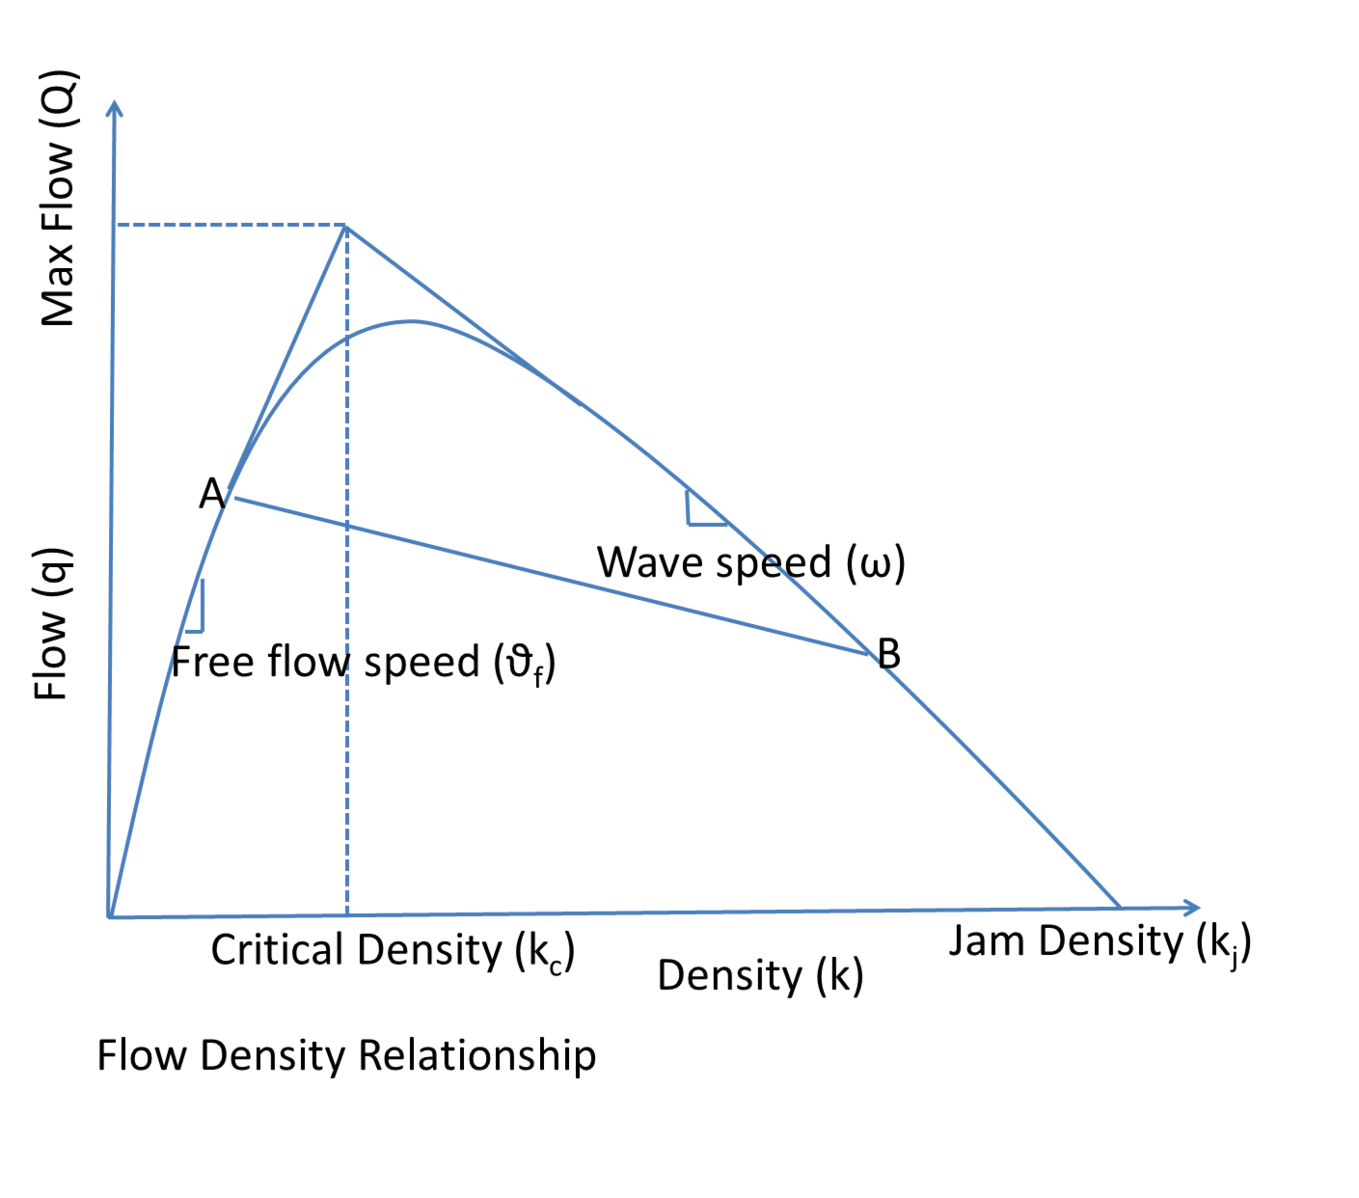
\includegraphics[width=0.9\textwidth]{Flow_Density_Relationship}
    \caption{Hidden-Layer Darstellung.}
    \label{fig:hidden-layers}
\end{figure}
